\documentclass[12pt,a4paper]{article}
\usepackage[UTF8]{ctex}
\usepackage{amsmath}
\usepackage{amssymb}
\usepackage{amsthm}
\usepackage{graphicx}
\usepackage{hyperref}
\usepackage{geometry}
\usepackage{algorithm}
\usepackage{algorithmic}
\usepackage{bm}
\usepackage{listings}
\usepackage{xcolor}
\usepackage{fancyhdr}
\geometry{left=2cm,right=2cm,top=2.5cm,bottom=2.5cm,headheight=15pt}
\setlength{\baselineskip}{1.1\baselineskip}
\setlength{\parskip}{0.5em}

% 导入通用样式
% 通用样式文件 - 统一所有文档的样式

% 目录样式设置 - 干净简洁,无边框,优化编号
% 使用基本 LaTeX 命令美化目录
\makeatletter
\renewcommand\@dotsep{2}
% 优化编号格式:减少缩进,使编号更紧凑
\renewcommand\l@section{\@dottedtocline{1}{0em}{1.2em}}
\renewcommand\l@subsection{\@dottedtocline{2}{1.2em}{1.8em}}
\renewcommand\l@subsubsection{\@dottedtocline{3}{3em}{2.2em}}
% 设置目录深度为3,显示到subsubsection级别
\setcounter{tocdepth}{3}
\makeatother

% 超链接设置 - 目录链接无颜色框
\hypersetup{
    colorlinks=true,
    linkcolor=black,          % 目录链接为黑色
    filecolor=black,
    urlcolor=blue,
    citecolor=black,
    pdfstartview=FitH,
    pdfborder={0 0 0},        % 无边框
    linkbordercolor={0 0 0},  % 链接边框颜色为黑色(不可见)
    pdfborderstyle={/S/U},    % 无边框样式
}

% 页眉页脚设置(在文档中重新定义)
\usepackage{fancyhdr}
% 注意:每个文档需要在导入 common_style.tex 后设置自己的页眉页脚

% 章节格式 - 简洁美观(使用基本命令)
\makeatletter
\renewcommand\section{\@startsection {section}{1}{\z@}%
                                   {-3.5ex \@plus -1ex \@minus -.2ex}%
                                   {2.3ex \@plus.2ex}%
                                   {\normalfont\Large\bfseries}}
\renewcommand\subsection{\@startsection{subsection}{2}{\z@}%
                                     {-3.25ex\@plus -1ex \@minus -.2ex}%
                                     {1.5ex \@plus .2ex}%
                                     {\normalfont\large\bfseries}}
\renewcommand\subsubsection{\@startsection{subsubsection}{3}{\z@}%
                                     {-3.25ex\@plus -1ex \@minus -.2ex}%
                                     {1.5ex \@plus .2ex}%
                                     {\normalfont\normalsize\bfseries}}
\makeatother

% 代码样式设置 - 简洁干净,无背景色
\definecolor{codegray}{rgb}{0.5,0.5,0.5}
\definecolor{keywordblue}{rgb}{0,0,0.8}
\definecolor{stringred}{rgb}{0.3,0.3,0.3}
\definecolor{commentgreen}{rgb}{0,0.5,0}

\lstdefinestyle{pythonstyle}{
    language=Python,
    % 无背景色 - 使用白色背景,与文档背景一致
    commentstyle=\color{commentgreen},      % 注释不用斜体
    keywordstyle=\color{keywordblue}\bfseries,
    stringstyle=\color{stringred},
    basicstyle=\ttfamily\small,
    breakatwhitespace=false,
    breaklines=true,
    captionpos=b,
    keepspaces=true,
    numbers=none,                           % 不显示行号
    showspaces=false,
    showstringspaces=false,
    showtabs=false,
    tabsize=4,
    frame=single,                          % 保留边框,但更简洁
    rulecolor=\color{black},
    framerule=0.5pt,                       % 细边框
    framexleftmargin=8pt,                  % 左边距(代码与左边框的距离)
    framexrightmargin=8pt,                 % 右边距(代码与右边框的距离)
    framextopmargin=6pt,                   % 上边距(代码与上边框的距离)
    framexbottommargin=6pt,                % 下边距(代码与下边框的距离)
    morekeywords={import,from,as,class,def,return,yield,lambda,if,elif,else,for,while,break,continue,pass,try,except,finally,raise,assert,with,del,global,nonlocal,and,or,not,in,is},
    identifierstyle=\color{black},
}

\lstset{style=pythonstyle}

% 封面宏定义
\newcommand{\makecover}[5]{%
    \newpage
    \thispagestyle{empty}
    \vspace*{1.5cm}
    \begin{center}
        \vspace{2cm}
        {\fontsize{48}{58}\selectfont\bfseries #1}\\[0.8cm]
        \vspace{1.5cm}
        {\Large #2}\\[0.4cm]
        \vspace{1.5cm}
        {\large #3}\\[1.5cm]
        
        % 神经网络图 - 紧凑版本,无标签
        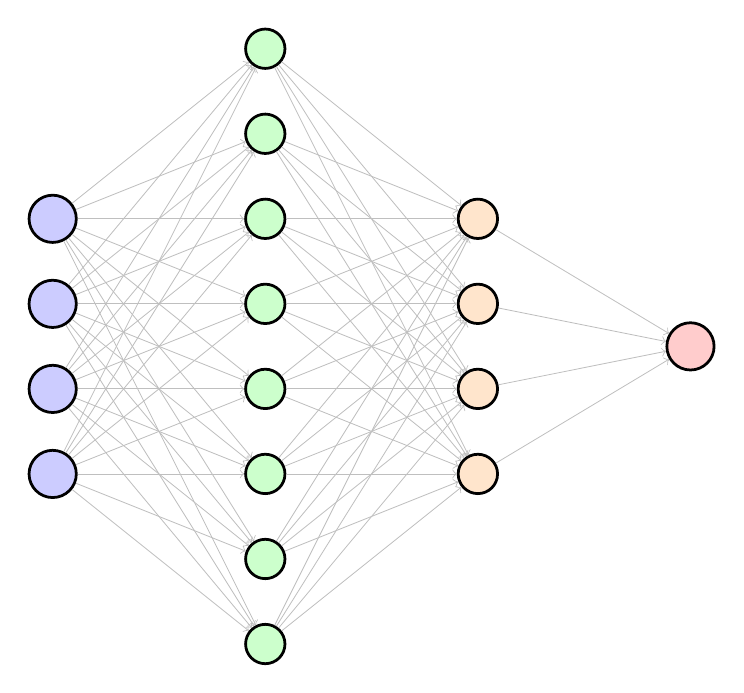
\begin{tikzpicture}[scale=0.9]
        % 定义神经元间距
        \def\spacing{1.2}
        
        % 输入层 - 4个神经元,关于横轴对称
        \node[circle, draw, minimum size=0.6cm, fill=blue!20, line width=1pt] (x1) at (0, -1.8) {};
        \node[circle, draw, minimum size=0.6cm, fill=blue!20, line width=1pt] (x2) at (0, -0.6) {};
        \node[circle, draw, minimum size=0.6cm, fill=blue!20, line width=1pt] (x3) at (0, 0.6) {};
        \node[circle, draw, minimum size=0.6cm, fill=blue!20, line width=1pt] (x4) at (0, 1.8) {};
        
        % 隐藏层1 - 8个神经元,关于横轴对称
        \node[circle, draw, minimum size=0.5cm, fill=green!20, line width=1pt] (h11) at (3, -4.2) {};
        \node[circle, draw, minimum size=0.5cm, fill=green!20, line width=1pt] (h12) at (3, -3.0) {};
        \node[circle, draw, minimum size=0.5cm, fill=green!20, line width=1pt] (h13) at (3, -1.8) {};
        \node[circle, draw, minimum size=0.5cm, fill=green!20, line width=1pt] (h14) at (3, -0.6) {};
        \node[circle, draw, minimum size=0.5cm, fill=green!20, line width=1pt] (h15) at (3, 0.6) {};
        \node[circle, draw, minimum size=0.5cm, fill=green!20, line width=1pt] (h16) at (3, 1.8) {};
        \node[circle, draw, minimum size=0.5cm, fill=green!20, line width=1pt] (h17) at (3, 3.0) {};
        \node[circle, draw, minimum size=0.5cm, fill=green!20, line width=1pt] (h18) at (3, 4.2) {};
        
        % 隐藏层2 - 4个神经元,关于横轴对称
        \node[circle, draw, minimum size=0.5cm, fill=orange!20, line width=1pt] (h21) at (6, -1.8) {};
        \node[circle, draw, minimum size=0.5cm, fill=orange!20, line width=1pt] (h22) at (6, -0.6) {};
        \node[circle, draw, minimum size=0.5cm, fill=orange!20, line width=1pt] (h23) at (6, 0.6) {};
        \node[circle, draw, minimum size=0.5cm, fill=orange!20, line width=1pt] (h24) at (6, 1.8) {};
        
        % 输出层 - 1个神经元,在横轴上
        \node[circle, draw, minimum size=0.6cm, fill=red!20, line width=1pt] (y) at (9, 0) {};
        
        % 输入层到隐藏层1的连接
        \foreach \i in {1,...,4}
            \foreach \j in {1,...,8}
                \draw[->, gray!50, line width=0.3pt] (x\i) -- (h1\j);
        
        % 隐藏层1到隐藏层2的连接
        \foreach \i in {1,...,8}
            \foreach \j in {1,...,4}
                \draw[->, gray!50, line width=0.3pt] (h1\i) -- (h2\j);
        
        % 隐藏层2到输出层的连接
        \foreach \i in {1,...,4}
            \draw[->, gray!50, line width=0.3pt] (h2\i) -- (y);
        \end{tikzpicture}
        
        \vfill
        \vspace{2cm}
        {\normalsize #5}
        \vspace{1.5cm}
    \end{center}
    \newpage
}



% 页眉页脚设置
\pagestyle{fancy}
\fancyhf{}
\fancyhead[L]{\leftmark}
\fancyhead[R]{\thepage}
\fancyfoot[C]{\small AI 相关数学理论基础}
\renewcommand{\headrulewidth}{0.3pt}
\renewcommand{\footrulewidth}{0.3pt}

\title{AI 相关数学理论基础}
\author{}
\date{\today}

\newtheorem{definition}{定义}[section]
\newtheorem{theorem}{定理}[section]
\newtheorem{proposition}{命题}[section]
\newtheorem{example}{例}[section]
\newtheorem{remark}{注}[section]

\begin{document}

% 封面
\makecover{AI 相关数学理论基础}{线性代数 · 概率论 · 优化理论 · 信息论 · 图论}{为人工智能和机器学习提供坚实的数学基础}{AI/ML 系列教程}

\maketitle

\tableofcontents
\newpage

\part{第一部分:线性代数与概率论}

\section{引言}

数学是人工智能和机器学习的理论基础,为算法设计、模型构建和性能分析提供了严格的数学框架。从线性代数到概率论,从优化理论到信息论,数学工具贯穿于 AI 研究的各个层面。

\textbf{数学在 AI 中的核心作用}:
\begin{itemize}
    \item \textbf{数据表示}:线性代数提供了向量和矩阵等数据结构,用于表示高维数据
    \item \textbf{不确定性建模}:概率论和统计学提供了处理不确定性和噪声的数学工具
    \item \textbf{模型优化}:优化理论提供了寻找最优参数的方法
    \item \textbf{信息度量}:信息论提供了量化信息和不确定性的方法
    \item \textbf{关系建模}:图论提供了表示和处理复杂关系结构的数学框架
\end{itemize}

本文档系统性地介绍 AI 领域中最常用的数学理论和方法,涵盖线性代数、概率论与统计学、优化理论、信息论和图论等核心内容。每个概念都配有清晰的定义、数学表达式、在 AI/ML 中的应用场景,以及生动的比喻帮助理解。

\section{线性代数基础}

线性代数是机器学习的数学语言,提供了表示和处理高维数据的工具。从数据表示到模型计算,线性代数无处不在。

\subsection{向量空间}

\begin{definition}[向量空间]
设 $V$ 是一个非空集合,$\mathbb{F}$ 是一个数域(通常是实数域 $\mathbb{R}$ 或复数域 $\mathbb{C}$)。如果 $V$ 上定义了加法和数乘运算,且满足以下8条公理,则称 $V$ 为 $\mathbb{F}$ 上的向量空间:
\begin{enumerate}
    \item 加法交换律:$\mathbf{u} + \mathbf{v} = \mathbf{v} + \mathbf{u}$
    \item 加法结合律:$(\mathbf{u} + \mathbf{v}) + \mathbf{w} = \mathbf{u} + (\mathbf{v} + \mathbf{w})$
    \item 存在零向量:$\mathbf{0} + \mathbf{v} = \mathbf{v}$
    \item 存在负向量:$\mathbf{v} + (-\mathbf{v}) = \mathbf{0}$
    \item 数乘单位元:$1 \cdot \mathbf{v} = \mathbf{v}$
    \item 数乘结合律:$(ab)\mathbf{v} = a(b\mathbf{v})$
    \item 数乘分配律1:$a(\mathbf{u} + \mathbf{v}) = a\mathbf{u} + a\mathbf{v}$
    \item 数乘分配律2:$(a + b)\mathbf{v} = a\mathbf{v} + b\mathbf{v}$
\end{enumerate}
\end{definition}

\textbf{通俗解释}:向量空间就像一个"数学宇宙",其中的"点"(向量)可以相加、可以伸缩,但必须遵循特定的规则。就像在三维空间中,我们可以将两个箭头相加,也可以将箭头拉长或缩短。

\textbf{在 AI/ML 中的应用}:
\begin{itemize}
    \item \textbf{特征空间}:在机器学习中,每个样本可以表示为一个向量,所有样本构成一个向量空间(特征空间)
    \item \textbf{词嵌入空间}:在自然语言处理中,词嵌入将词汇映射到高维向量空间,语义相似的词在空间中距离较近
    \item \textbf{图像表示}:图像可以展平为向量,所有可能的图像构成一个巨大的向量空间
\end{itemize}

\begin{example}[图像特征空间]
一张 $28 \times 28$ 的灰度图像可以表示为一个 $784$ 维向量 $\mathbf{x} \in \mathbb{R}^{784}$。所有可能的图像构成一个 $784$ 维的向量空间。在这个空间中,相似的图像(如都是手写数字"5")会聚集在一起。
\end{example}

\subsection{矩阵运算}

矩阵是线性代数中的核心对象,用于表示线性变换和存储数据。

\begin{definition}[矩阵]
一个 $m \times n$ 矩阵 $\mathbf{A}$ 是一个由 $m$ 行 $n$ 列元素排列成的矩形阵列:
\begin{equation}
\mathbf{A} = \begin{bmatrix}
a_{11} & a_{12} & \cdots & a_{1n} \\
a_{21} & a_{22} & \cdots & a_{2n} \\
\vdots & \vdots & \ddots & \vdots \\
a_{m1} & a_{m2} & \cdots & a_{mn}
\end{bmatrix} \in \mathbb{R}^{m \times n}
\end{equation}
\end{definition}

\textbf{矩阵乘法}:对于矩阵 $\mathbf{A} \in \mathbb{R}^{m \times n}$ 和 $\mathbf{B} \in \mathbb{R}^{n \times p}$,其乘积 $\mathbf{C} = \mathbf{A}\mathbf{B} \in \mathbb{R}^{m \times p}$ 定义为:
\begin{equation}
c_{ij} = \sum_{k=1}^n a_{ik} b_{kj}
\end{equation}

\textbf{矩阵转置}:矩阵 $\mathbf{A}$ 的转置 $\mathbf{A}^T$ 定义为:
\begin{equation}
(\mathbf{A}^T)_{ij} = a_{ji}
\end{equation}

\textbf{矩阵的逆}:对于方阵 $\mathbf{A} \in \mathbb{R}^{n \times n}$,如果存在矩阵 $\mathbf{A}^{-1}$ 使得 $\mathbf{A}\mathbf{A}^{-1} = \mathbf{A}^{-1}\mathbf{A} = \mathbf{I}$(单位矩阵),则称 $\mathbf{A}$ 可逆,$\mathbf{A}^{-1}$ 为其逆矩阵。

\textbf{在 AI/ML 中的应用}:
\begin{itemize}
    \item \textbf{神经网络计算}:前向传播本质上是矩阵乘法,$\mathbf{y} = \mathbf{W}\mathbf{x} + \mathbf{b}$
    \item \textbf{数据变换}:主成分分析(PCA)使用矩阵分解降维
    \item \textbf{图像处理}:卷积操作可以表示为矩阵乘法
    \item \textbf{推荐系统}:用户-物品评分矩阵用于协同过滤
\end{itemize}

\begin{example}[神经网络中的矩阵乘法]
在多层感知机中,第 $l$ 层的计算可以表示为:
\begin{equation}
\mathbf{h}^{(l)} = \sigma(\mathbf{W}^{(l)} \mathbf{h}^{(l-1)} + \mathbf{b}^{(l)})
\end{equation}
其中,$\mathbf{W}^{(l)} \in \mathbb{R}^{n_l \times n_{l-1}}$ 是权重矩阵,$\mathbf{h}^{(l-1)} \in \mathbb{R}^{n_{l-1}}$ 是上一层的输出,$\sigma$ 是激活函数。矩阵乘法 $\mathbf{W}^{(l)} \mathbf{h}^{(l-1)}$ 计算了所有神经元之间的连接。
\end{example}

\subsection{特征值与特征向量}

特征值和特征向量揭示了矩阵的本质结构,在降维、主成分分析等领域有重要应用。

\begin{definition}[特征值与特征向量]
对于方阵 $\mathbf{A} \in \mathbb{R}^{n \times n}$,如果存在标量 $\lambda$ 和非零向量 $\mathbf{v}$ 使得:
\begin{equation}
\mathbf{A}\mathbf{v} = \lambda \mathbf{v}
\end{equation}
则称 $\lambda$ 为 $\mathbf{A}$ 的特征值,$\mathbf{v}$ 为对应的特征向量。
\end{definition}

\textbf{特征值分解}:如果矩阵 $\mathbf{A}$ 有 $n$ 个线性无关的特征向量,则可以分解为:
\begin{equation}
\mathbf{A} = \mathbf{V}\boldsymbol{\Lambda}\mathbf{V}^{-1}
\end{equation}
其中,$\mathbf{V}$ 的列是特征向量,$\boldsymbol{\Lambda}$ 是对角矩阵,对角线元素是特征值。

\textbf{奇异值分解(SVD)}:对于任意矩阵 $\mathbf{A} \in \mathbb{R}^{m \times n}$,可以分解为:
\begin{equation}
\mathbf{A} = \mathbf{U}\boldsymbol{\Sigma}\mathbf{V}^T
\end{equation}
其中,$\mathbf{U} \in \mathbb{R}^{m \times m}$ 和 $\mathbf{V} \in \mathbb{R}^{n \times n}$ 是正交矩阵,$\boldsymbol{\Sigma} \in \mathbb{R}^{m \times n}$ 是对角矩阵(奇异值矩阵)。

\textbf{通俗解释}:特征向量是矩阵作用下的"不变方向",特征值表示在这个方向上的"伸缩倍数"。就像拉伸一个弹性物体,有些方向会被拉伸(特征值大于1),有些方向会被压缩(特征值小于1),而特征向量就是这些特殊的方向。

\textbf{在 AI/ML 中的应用}:
\begin{itemize}
    \item \textbf{主成分分析(PCA)}:使用特征值分解找到数据的主要变化方向
    \item \textbf{降维}:保留最大的几个特征值对应的特征向量,实现数据降维
    \item \textbf{推荐系统}:SVD 用于矩阵分解,发现潜在因子
    \item \textbf{图像压缩}:使用 SVD 压缩图像数据
    \item \textbf{自然语言处理}:潜在语义分析(LSA)使用 SVD
\end{itemize}

\begin{example}[主成分分析]
给定数据矩阵 $\mathbf{X} \in \mathbb{R}^{n \times d}$($n$ 个样本,$d$ 个特征),PCA 的步骤如下:
\begin{enumerate}
    \item 中心化数据:$\tilde{\mathbf{X}} = \mathbf{X} - \bar{\mathbf{X}}$
    \item 计算协方差矩阵:$\mathbf{C} = \frac{1}{n-1}\tilde{\mathbf{X}}^T\tilde{\mathbf{X}}$
    \item 特征值分解:$\mathbf{C} = \mathbf{V}\boldsymbol{\Lambda}\mathbf{V}^T$
    \item 选择前 $k$ 个最大特征值对应的特征向量,构成投影矩阵 $\mathbf{W} \in \mathbb{R}^{d \times k}$
    \item 降维:$\mathbf{Y} = \tilde{\mathbf{X}}\mathbf{W}$
\end{enumerate}
主成分就是协方差矩阵的特征向量,特征值表示该方向上的方差大小。
\end{example}

\subsection{范数与距离}

范数用于度量向量的大小,距离用于度量向量之间的差异。

\begin{definition}[向量范数]
向量 $\mathbf{x} \in \mathbb{R}^n$ 的 $p$-范数定义为:
\begin{equation}
\|\mathbf{x}\|_p = \left(\sum_{i=1}^n |x_i|^p\right)^{1/p}
\end{equation}

常用的范数:
\begin{itemize}
    \item $L_1$ 范数(曼哈顿距离):$\|\mathbf{x}\|_1 = \sum_{i=1}^n |x_i|$
    \item $L_2$ 范数(欧氏距离):$\|\mathbf{x}\|_2 = \sqrt{\sum_{i=1}^n x_i^2}$
    \item $L_\infty$ 范数:$\|\mathbf{x}\|_\infty = \max_i |x_i|$
\end{itemize}
\end{definition}

\textbf{距离度量}:两个向量 $\mathbf{x}, \mathbf{y} \in \mathbb{R}^n$ 之间的距离:
\begin{itemize}
    \item 欧氏距离:$d_2(\mathbf{x}, \mathbf{y}) = \|\mathbf{x} - \mathbf{y}\|_2$
    \item 曼哈顿距离:$d_1(\mathbf{x}, \mathbf{y}) = \|\mathbf{x} - \mathbf{y}\|_1$
    \item 余弦相似度:$\cos(\theta) = \frac{\mathbf{x}^T\mathbf{y}}{\|\mathbf{x}\|_2 \|\mathbf{y}\|_2}$
\end{itemize}

\textbf{在 AI/ML 中的应用}:
\begin{itemize}
    \item \textbf{正则化}:$L_1$ 正则化(Lasso)和 $L_2$ 正则化(Ridge)用于防止过拟合
    \item \textbf{聚类}:K-means 使用欧氏距离度量样本相似性
    \item \textbf{相似度计算}:余弦相似度用于文本相似度、推荐系统
    \item \textbf{损失函数}:均方误差使用 $L_2$ 范数,平均绝对误差使用 $L_1$ 范数
\end{itemize}

\subsubsection{线性代数在神经网络中的应用}

\textbf{前向传播的矩阵表示}:

在神经网络中,每一层的计算都可以表示为矩阵乘法:

\begin{equation}
\mathbf{h}^{(l)} = \sigma(\mathbf{W}^{(l)} \mathbf{h}^{(l-1)} + \mathbf{b}^{(l)})
\end{equation}

其中:
\begin{itemize}
    \item $\mathbf{W}^{(l)} \in \mathbb{R}^{d_l \times d_{l-1}}$:第 $l$ 层的权重矩阵
    \item $\mathbf{h}^{(l-1)} \in \mathbb{R}^{d_{l-1}}$:第 $l-1$ 层的输出(第 $l$ 层的输入)
    \item $\mathbf{b}^{(l)} \in \mathbb{R}^{d_l}$:偏置向量
    \item $\sigma(\cdot)$:激活函数
\end{itemize}

\textbf{批量处理}:

对于批量大小为 $B$ 的输入,可以并行计算:

\begin{equation}
\mathbf{H}^{(l)} = \sigma(\mathbf{W}^{(l)} \mathbf{H}^{(l-1)} + \mathbf{b}^{(l)} \mathbf{1}^T)
\end{equation}

其中 $\mathbf{H}^{(l)} \in \mathbb{R}^{d_l \times B}$ 是批量输出矩阵,$\mathbf{1} \in \mathbb{R}^B$ 是全1向量。

\textbf{在 LLM 中的应用}:

\textbf{注意力机制中的矩阵运算}:

Transformer 中的缩放点积注意力可以表示为:

\begin{equation}
\text{Attention}(\mathbf{Q}, \mathbf{K}, \mathbf{V}) = \text{softmax}\left(\frac{\mathbf{Q}\mathbf{K}^T}{\sqrt{d_k}}\right)\mathbf{V}
\end{equation}

其中:
\begin{itemize}
    \item $\mathbf{Q} \in \mathbb{R}^{n \times d_k}$:查询矩阵
    \item $\mathbf{K} \in \mathbb{R}^{m \times d_k}$:键矩阵
    \item $\mathbf{V} \in \mathbb{R}^{m \times d_v}$:值矩阵
    \item $\mathbf{Q}\mathbf{K}^T$:计算注意力分数矩阵($n \times m$)
    \item 矩阵乘法的复杂度:$O(n \cdot m \cdot d_k)$
\end{itemize}

\textbf{多头注意力的矩阵分割}:

在多头注意力中,通过矩阵重塑实现并行计算:

\begin{align}
\mathbf{Q} &\rightarrow [\mathbf{Q}_1, \mathbf{Q}_2, \ldots, \mathbf{Q}_h] \quad \text{(分割为 $h$ 个头)} \\
\text{head}_i &= \text{Attention}(\mathbf{Q}_i, \mathbf{K}_i, \mathbf{V}_i) \\
\text{MultiHead} &= \text{Concat}(\text{head}_1, \ldots, \text{head}_h) \mathbf{W}^O
\end{align}

这种设计充分利用了矩阵运算的并行性,是现代 GPU 加速的基础。

\section{概率论与统计学}

概率论和统计学为机器学习提供了处理不确定性的数学框架,从数据分布建模到参数估计,都离不开概率统计方法。

\subsection{概率分布}

概率分布描述了随机变量的取值规律,是统计学习的基础。

\begin{definition}[随机变量与概率分布]
随机变量 $X$ 是一个函数,将样本空间映射到实数集。概率分布函数 $P(X = x)$ 或概率密度函数 $p(x)$ 描述了随机变量取各个值的概率。
\end{definition}

\textbf{离散分布}:

\textbf{伯努利分布}:单次试验的成功概率分布
\begin{equation}
P(X = k) = \begin{cases}
p & \text{if } k = 1 \\
1-p & \text{if } k = 0
\end{cases}
\end{equation}
期望:$\mathbb{E}[X] = p$,方差:$\text{Var}(X) = p(1-p)$

\textbf{二项分布}:$n$ 次独立伯努利试验的成功次数
\begin{equation}
P(X = k) = \binom{n}{k} p^k (1-p)^{n-k}, \quad k = 0, 1, \ldots, n
\end{equation}
期望:$\mathbb{E}[X] = np$,方差:$\text{Var}(X) = np(1-p)$

\textbf{多项分布}:$n$ 次独立试验中各类别出现的次数
\begin{equation}
P(X_1 = k_1, \ldots, X_m = k_m) = \frac{n!}{k_1! \cdots k_m!} p_1^{k_1} \cdots p_m^{k_m}
\end{equation}
其中,$\sum_{i=1}^m k_i = n$,$\sum_{i=1}^m p_i = 1$。

\textbf{连续分布}:

\textbf{正态分布(高斯分布)}:
\begin{equation}
p(x) = \frac{1}{\sqrt{2\pi\sigma^2}} \exp\left(-\frac{(x-\mu)^2}{2\sigma^2}\right)
\end{equation}
记作 $X \sim \mathcal{N}(\mu, \sigma^2)$,其中 $\mu$ 是均值,$\sigma^2$ 是方差。

\textbf{多元正态分布}:
\begin{equation}
p(\mathbf{x}) = \frac{1}{(2\pi)^{d/2}|\boldsymbol{\Sigma}|^{1/2}} \exp\left(-\frac{1}{2}(\mathbf{x}-\boldsymbol{\mu})^T\boldsymbol{\Sigma}^{-1}(\mathbf{x}-\boldsymbol{\mu})\right)
\end{equation}
其中,$\boldsymbol{\mu}$ 是均值向量,$\boldsymbol{\Sigma}$ 是协方差矩阵。

\textbf{在 AI/ML 中的应用}:
\begin{itemize}
    \item \textbf{分类问题}:多项分布用于多分类,伯努利分布用于二分类
    \item \textbf{回归问题}:假设误差服从正态分布,使用最大似然估计
    \item \textbf{生成模型}:变分自编码器(VAE)、生成对抗网络(GAN)使用概率分布
    \item \textbf{贝叶斯方法}:使用先验分布和似然函数进行推理
\end{itemize}

\begin{example}[逻辑回归中的概率建模]
在逻辑回归中,假设 $P(Y=1|\mathbf{x}) = \sigma(\mathbf{w}^T\mathbf{x} + b)$,其中 $\sigma$ 是 sigmoid 函数。这实际上是在建模 $Y$ 服从伯努利分布,参数为 $\sigma(\mathbf{w}^T\mathbf{x} + b)$。
\end{example}

\subsection{贝叶斯定理}

贝叶斯定理是概率推理的核心,提供了在观察到新证据后更新信念的方法。

\begin{theorem}[贝叶斯定理]
对于事件 $A$ 和 $B$,如果 $P(B) > 0$,则:
\begin{equation}
P(A|B) = \frac{P(B|A)P(A)}{P(B)}
\end{equation}

在连续情况下,对于随机变量:
\begin{equation}
p(\theta|\mathbf{x}) = \frac{p(\mathbf{x}|\theta)p(\theta)}{p(\mathbf{x})} = \frac{p(\mathbf{x}|\theta)p(\theta)}{\int p(\mathbf{x}|\theta)p(\theta) d\theta}
\end{equation}
\end{theorem}

\textbf{术语解释}:
\begin{itemize}
    \item $P(\theta)$:先验概率(Prior),在观察到数据前的信念
    \item $P(\mathbf{x}|\theta)$:似然函数(Likelihood),给定参数下数据的概率
    \item $P(\theta|\mathbf{x})$:后验概率(Posterior),观察到数据后的信念
    \item $P(\mathbf{x})$:证据(Evidence),数据的边际概率
\end{itemize}

\textbf{通俗解释}:贝叶斯定理就像"根据结果反推原因"。比如,如果知道某种疾病的症状(结果),可以反推患病的概率(原因)。先验概率是"一般人群中患病的概率",后验概率是"出现症状后患病的概率"。

\textbf{在 AI/ML 中的应用}:
\begin{itemize}
    \item \textbf{朴素贝叶斯分类器}:用于文本分类、垃圾邮件检测
    \item \textbf{贝叶斯网络}:表示变量之间的条件依赖关系
    \item \textbf{贝叶斯优化}:用于超参数优化
    \item \textbf{变分推理}:近似计算后验分布
    \item \textbf{贝叶斯神经网络}:为权重分配概率分布,量化不确定性
\end{itemize}

\begin{example}[垃圾邮件分类]
假设:
\begin{itemize}
    \item $P(\text{垃圾邮件}) = 0.3$(先验)
    \item $P(\text{"免费"}|\text{垃圾邮件}) = 0.8$(似然)
    \item $P(\text{"免费"}|\text{正常邮件}) = 0.1$
\end{itemize}

如果一封邮件包含"免费",则:
\begin{align}
P(\text{垃圾邮件}|\text{"免费"}) &= \frac{P(\text{"免费"}|\text{垃圾邮件})P(\text{垃圾邮件})}{P(\text{"免费"})} \\
&= \frac{0.8 \times 0.3}{0.8 \times 0.3 + 0.1 \times 0.7} = \frac{0.24}{0.31} \approx 0.77
\end{align}
因此,这封邮件是垃圾邮件的概率约为 77\%。
\end{example}

\subsection{最大似然估计}

最大似然估计(Maximum Likelihood Estimation, MLE)是参数估计的重要方法。

\begin{definition}[最大似然估计]
给定独立同分布的样本 $\mathbf{x}_1, \mathbf{x}_2, \ldots, \mathbf{x}_n$,其联合概率密度为 $p(\mathbf{x}_1, \ldots, \mathbf{x}_n|\theta) = \prod_{i=1}^n p(\mathbf{x}_i|\theta)$。似然函数定义为:
\begin{equation}
L(\theta) = \prod_{i=1}^n p(\mathbf{x}_i|\theta)
\end{equation}

对数似然函数为:
\begin{equation}
\ell(\theta) = \log L(\theta) = \sum_{i=1}^n \log p(\mathbf{x}_i|\theta)
\end{equation}

最大似然估计 $\hat{\theta}_{MLE}$ 是使似然函数最大的参数值:
\begin{equation}
\hat{\theta}_{MLE} = \arg\max_\theta L(\theta) = \arg\max_\theta \ell(\theta)
\end{equation}
\end{definition}

\textbf{求解方法}:通常对对数似然函数求导并令其为零:
\begin{equation}
\frac{\partial \ell(\theta)}{\partial \theta} = 0
\end{equation}

\textbf{在 AI/ML 中的应用}:
\begin{itemize}
    \item \textbf{线性回归}:假设误差服从正态分布,MLE 等价于最小二乘法
    \item \textbf{逻辑回归}:使用 MLE 估计参数
    \item \textbf{神经网络}:交叉熵损失函数对应多项分布的 MLE
    \item \textbf{高斯混合模型}:使用 EM 算法进行 MLE
\end{itemize}

\begin{example}[正态分布的 MLE]
假设样本 $x_1, \ldots, x_n$ 来自正态分布 $\mathcal{N}(\mu, \sigma^2)$,则:
\begin{align}
\ell(\mu, \sigma^2) &= \sum_{i=1}^n \log \left[\frac{1}{\sqrt{2\pi\sigma^2}} \exp\left(-\frac{(x_i-\mu)^2}{2\sigma^2}\right)\right] \\
&= -\frac{n}{2}\log(2\pi\sigma^2) - \frac{1}{2\sigma^2}\sum_{i=1}^n (x_i-\mu)^2
\end{align}

对 $\mu$ 和 $\sigma^2$ 求导并令其为零:
\begin{align}
\frac{\partial \ell}{\partial \mu} &= \frac{1}{\sigma^2}\sum_{i=1}^n (x_i-\mu) = 0 \Rightarrow \hat{\mu} = \frac{1}{n}\sum_{i=1}^n x_i \\
\frac{\partial \ell}{\partial \sigma^2} &= -\frac{n}{2\sigma^2} + \frac{1}{2(\sigma^2)^2}\sum_{i=1}^n (x_i-\mu)^2 = 0 \Rightarrow \hat{\sigma}^2 = \frac{1}{n}\sum_{i=1}^n (x_i-\hat{\mu})^2
\end{align}

因此,样本均值和样本方差分别是均值和方差的最大似然估计。
\end{example}

\subsection{期望、方差与协方差}

这些统计量描述了随机变量的重要特征。

\begin{definition}[期望]
离散随机变量 $X$ 的期望:
\begin{equation}
\mathbb{E}[X] = \sum_x x P(X = x)
\end{equation}

连续随机变量 $X$ 的期望:
\begin{equation}
\mathbb{E}[X] = \int_{-\infty}^{\infty} x p(x) dx
\end{equation}
\end{definition}

\begin{definition}[方差]
随机变量 $X$ 的方差:
\begin{equation}
\text{Var}(X) = \mathbb{E}[(X - \mathbb{E}[X])^2] = \mathbb{E}[X^2] - (\mathbb{E}[X])^2
\end{equation}
\end{definition}

\begin{definition}[协方差]
两个随机变量 $X$ 和 $Y$ 的协方差:
\begin{equation}
\text{Cov}(X, Y) = \mathbb{E}[(X - \mathbb{E}[X])(Y - \mathbb{E}[Y])] = \mathbb{E}[XY] - \mathbb{E}[X]\mathbb{E}[Y]
\end{equation}
\end{definition}

\textbf{在 AI/ML 中的应用}:
\begin{itemize}
    \item \textbf{特征选择}:使用方差筛选低方差特征
    \item \textbf{主成分分析}:协方差矩阵的特征值分解
    \item \textbf{批量归一化}:归一化均值和方差
    \item \textbf{损失函数}:均方误差是方差的估计
\end{itemize}

\part{第二部分:优化理论与信息论}

\subsubsection{概率分布在机器学习中的应用}

\textbf{高斯分布在回归问题中的应用}:

线性回归假设误差服从高斯分布:

\begin{equation}
y = \mathbf{w}^T \mathbf{x} + b + \epsilon, \quad \epsilon \sim \mathcal{N}(0, \sigma^2)
\end{equation}

这导致最大似然估计等价于最小化均方误差(MSE):

\begin{equation}
\mathcal{L}(\mathbf{w}, b) = \frac{1}{n}\sum_{i=1}^n (y_i - \mathbf{w}^T \mathbf{x}_i - b)^2
\end{equation}

\textbf{多项分布在分类问题中的应用}:

多分类问题中,softmax 函数将 logits 转换为概率分布:

\begin{equation}
P(y = k | \mathbf{x}) = \frac{\exp(z_k)}{\sum_{j=1}^C \exp(z_j)} = \text{softmax}(\mathbf{z})_k
\end{equation}

其中 $\mathbf{z} = [z_1, z_2, \ldots, z_C]^T$ 是模型的原始输出(logits),$C$ 是类别数。

\textbf{在 LLM 中的应用}:

\textbf{语言模型的概率建模}:

自回归语言模型(如 GPT)将文本生成建模为条件概率:

\begin{equation}
P(w_1, w_2, \ldots, w_n) = \prod_{i=1}^n P(w_i | w_1, w_2, \ldots, w_{i-1})
\end{equation}

每一步生成都是基于前面所有词的条件概率分布:

\begin{equation}
P(w_i | w_{<i}) = \text{softmax}(\mathbf{W} \mathbf{h}_i)
\end{equation}

其中 $\mathbf{h}_i$ 是位置 $i$ 的隐藏状态,$\mathbf{W}$ 是输出投影矩阵。

\textbf{困惑度(Perplexity)}:

困惑度是语言模型的重要评估指标,定义为:

\begin{equation}
\text{Perplexity} = \exp\left(-\frac{1}{n}\sum_{i=1}^n \log P(w_i | w_{<i})\right)
\end{equation}

困惑度越小,模型对序列的预测越确定,性能越好。

\section{优化理论}

优化理论提供了寻找函数最小值或最大值的方法,是机器学习算法训练的核心。

\subsection{梯度下降}

梯度下降是最基本的优化算法,通过沿着梯度的反方向迭代更新参数。

\begin{definition}[梯度]
对于多元函数 $f(\mathbf{x}): \mathbb{R}^n \to \mathbb{R}$,其梯度定义为:
\begin{equation}
\nabla f(\mathbf{x}) = \left[\frac{\partial f}{\partial x_1}, \frac{\partial f}{\partial x_2}, \ldots, \frac{\partial f}{\partial x_n}\right]^T
\end{equation}

梯度指向函数值增加最快的方向。
\end{definition}

\textbf{梯度下降算法}:
\begin{algorithm}
\caption{梯度下降算法}
\begin{algorithmic}[1]
\REQUIRE 目标函数 $f(\mathbf{x})$,学习率 $\eta > 0$,初始点 $\mathbf{x}_0$
\ENSURE 局部最优解 $\mathbf{x}^*$
\STATE 初始化 $\mathbf{x} = \mathbf{x}_0$
\REPEAT
    \STATE 计算梯度:$\mathbf{g} = \nabla f(\mathbf{x})$
    \STATE 更新参数:$\mathbf{x} \leftarrow \mathbf{x} - \eta \mathbf{g}$
\UNTIL{收敛(如 $\|\mathbf{g}\| < \epsilon$)}
\end{algorithmic}
\end{algorithm}

\textbf{学习率的选择}:
\begin{itemize}
    \item 学习率太小:收敛慢
    \item 学习率太大:可能发散,无法收敛
    \item 自适应学习率:Adam、RMSprop 等算法自动调整学习率
\end{itemize}

\textbf{在 AI/ML 中的应用}:
\begin{itemize}
    \item \textbf{神经网络训练}:反向传播算法使用梯度下降更新权重
    \item \textbf{线性回归}:最小化均方误差
    \item \textbf{逻辑回归}:最小化对数似然函数
    \item \textbf{所有监督学习算法}:本质上都是优化问题
\end{itemize}

\begin{example}[线性回归的梯度下降]
对于线性回归 $y = \mathbf{w}^T\mathbf{x} + b$,损失函数为:
\begin{equation}
\mathcal{L}(\mathbf{w}, b) = \frac{1}{2n}\sum_{i=1}^n (y_i - \mathbf{w}^T\mathbf{x}_i - b)^2
\end{equation}

梯度为:
\begin{align}
\frac{\partial \mathcal{L}}{\partial \mathbf{w}} &= -\frac{1}{n}\sum_{i=1}^n (y_i - \mathbf{w}^T\mathbf{x}_i - b)\mathbf{x}_i \\
\frac{\partial \mathcal{L}}{\partial b} &= -\frac{1}{n}\sum_{i=1}^n (y_i - \mathbf{w}^T\mathbf{x}_i - b)
\end{align}

梯度下降更新规则:
\begin{align}
\mathbf{w} &\leftarrow \mathbf{w} - \eta \frac{\partial \mathcal{L}}{\partial \mathbf{w}} \\
b &\leftarrow b - \eta \frac{\partial \mathcal{L}}{\partial b}
\end{align}
\end{example}

\subsection{凸优化}

凸优化问题具有良好的性质,可以保证找到全局最优解。

\begin{definition}[凸函数]
函数 $f: \mathbb{R}^n \to \mathbb{R}$ 是凸函数,如果对于任意 $\mathbf{x}_1, \mathbf{x}_2 \in \mathbb{R}^n$ 和 $\lambda \in [0, 1]$,有:
\begin{equation}
f(\lambda \mathbf{x}_1 + (1-\lambda)\mathbf{x}_2) \leq \lambda f(\mathbf{x}_1) + (1-\lambda) f(\mathbf{x}_2)
\end{equation}
\end{definition}

\textbf{凸优化问题}:
\begin{equation}
\begin{aligned}
\min_{\mathbf{x}} \quad & f(\mathbf{x}) \\
\text{s.t.} \quad & g_i(\mathbf{x}) \leq 0, \quad i = 1, \ldots, m \\
& h_j(\mathbf{x}) = 0, \quad j = 1, \ldots, p
\end{aligned}
\end{equation}
其中,$f$ 和 $g_i$ 是凸函数,$h_j$ 是仿射函数。

\textbf{凸优化的性质}:
\begin{itemize}
    \item 局部最优解就是全局最优解
    \item 可以使用高效的算法求解(如内点法)
    \item 对偶理论提供了另一种求解视角
\end{itemize}

\textbf{在 AI/ML 中的应用}:
\begin{itemize}
    \item \textbf{支持向量机(SVM)}:凸优化问题
    \item \textbf{逻辑回归}:凸优化问题(对数似然函数是凹函数,取负号后是凸函数)
    \item \textbf{Lasso 和 Ridge 回归}:凸优化问题
    \item \textbf{线性规划}:用于资源分配等问题
\end{itemize}

\subsubsection{梯度下降在机器学习中的应用}

\textbf{批量梯度下降(BGD)}:

对于损失函数 $\mathcal{L}(\theta) = \frac{1}{n}\sum_{i=1}^n \ell(f(\mathbf{x}_i; \theta), y_i)$,批量梯度下降的更新规则为:

\begin{equation}
\theta_{t+1} = \theta_t - \eta \nabla_\theta \mathcal{L}(\theta_t) = \theta_t - \frac{\eta}{n}\sum_{i=1}^n \nabla_\theta \ell(f(\mathbf{x}_i; \theta_t), y_i)
\end{equation}

\textbf{随机梯度下降(SGD)}:

每次只使用一个样本计算梯度:

\begin{equation}
\theta_{t+1} = \theta_t - \eta \nabla_\theta \ell(f(\mathbf{x}_i; \theta_t), y_i)
\end{equation}

\textbf{小批量梯度下降(Mini-batch GD)}:

使用小批量样本(通常 $B = 32, 64, 128$):

\begin{equation}
\theta_{t+1} = \theta_t - \frac{\eta}{B}\sum_{i \in \mathcal{B}_t} \nabla_\theta \ell(f(\mathbf{x}_i; \theta_t), y_i)
\end{equation}

\textbf{Adam 优化器}:

Adam 结合了动量和自适应学习率:

\begin{align}
\mathbf{m}_t &= \beta_1 \mathbf{m}_{t-1} + (1-\beta_1) \mathbf{g}_t \quad \text{(一阶矩估计)} \\
\mathbf{v}_t &= \beta_2 \mathbf{v}_{t-1} + (1-\beta_2) \mathbf{g}_t^2 \quad \text{(二阶矩估计)} \\
\hat{\mathbf{m}}_t &= \frac{\mathbf{m}_t}{1-\beta_1^t} \quad \text{(偏差修正)} \\
\hat{\mathbf{v}}_t &= \frac{\mathbf{v}_t}{1-\beta_2^t} \\
\theta_{t+1} &= \theta_t - \frac{\eta}{\sqrt{\hat{\mathbf{v}}_t} + \epsilon} \hat{\mathbf{m}}_t
\end{align}

其中 $\mathbf{g}_t = \nabla_\theta \mathcal{L}(\theta_t)$ 是梯度,$\beta_1 = 0.9$,$\beta_2 = 0.999$,$\epsilon = 10^{-8}$。

\textbf{在 LLM 训练中的应用}:

大语言模型的训练通常使用:
\begin{itemize}
    \item \textbf{混合精度训练}:使用 FP16 降低内存占用,FP32 保证数值稳定性
    \item \textbf{梯度累积}:当 GPU 内存有限时,累积多个小批量的梯度再更新
    \item \textbf{学习率调度}:使用 warmup 和学习率衰减策略
    \item \textbf{权重衰减}:$L_2$ 正则化防止过拟合
\end{itemize}

\subsection{拉格朗日乘数法}

拉格朗日乘数法用于求解带约束的优化问题。

\begin{theorem}[拉格朗日乘数法]
考虑优化问题:
\begin{equation}
\begin{aligned}
\min_{\mathbf{x}} \quad & f(\mathbf{x}) \\
\text{s.t.} \quad & g_i(\mathbf{x}) = 0, \quad i = 1, \ldots, m
\end{aligned}
\end{equation}

构造拉格朗日函数:
\begin{equation}
\mathcal{L}(\mathbf{x}, \boldsymbol{\lambda}) = f(\mathbf{x}) + \sum_{i=1}^m \lambda_i g_i(\mathbf{x})
\end{equation}

最优解满足:
\begin{align}
\nabla_{\mathbf{x}} \mathcal{L} &= \mathbf{0} \\
\nabla_{\boldsymbol{\lambda}} \mathcal{L} &= \mathbf{0}
\end{align}
即:
\begin{align}
\nabla f(\mathbf{x}) + \sum_{i=1}^m \lambda_i \nabla g_i(\mathbf{x}) &= \mathbf{0} \\
g_i(\mathbf{x}) &= 0, \quad i = 1, \ldots, m
\end{align}
\end{theorem}

\textbf{KKT 条件}:对于不等式约束,使用 Karush-Kuhn-Tucker (KKT) 条件:
\begin{align}
\nabla f(\mathbf{x}) + \sum_{i=1}^m \lambda_i \nabla g_i(\mathbf{x}) + \sum_{j=1}^p \nu_j \nabla h_j(\mathbf{x}) &= \mathbf{0} \\
g_i(\mathbf{x}) &\leq 0 \\
\lambda_i &\geq 0 \\
\lambda_i g_i(\mathbf{x}) &= 0
\end{align}

\textbf{在 AI/ML 中的应用}:
\begin{itemize}
    \item \textbf{支持向量机}:使用拉格朗日乘数法推导对偶问题
    \item \textbf{正则化}:可以看作带约束的优化问题
    \item \textbf{最大熵模型}:在约束条件下最大化熵
\end{itemize}

\begin{example}[支持向量机的对偶问题]
SVM 的原始问题:
\begin{equation}
\begin{aligned}
\min_{\mathbf{w}, b} \quad & \frac{1}{2}\|\mathbf{w}\|^2 \\
\text{s.t.} \quad & y_i(\mathbf{w}^T\mathbf{x}_i + b) \geq 1, \quad i = 1, \ldots, n
\end{aligned}
\end{equation}

拉格朗日函数:
\begin{equation}
\mathcal{L}(\mathbf{w}, b, \boldsymbol{\alpha}) = \frac{1}{2}\|\mathbf{w}\|^2 - \sum_{i=1}^n \alpha_i[y_i(\mathbf{w}^T\mathbf{x}_i + b) - 1]
\end{equation}

对偶问题:
\begin{equation}
\begin{aligned}
\max_{\boldsymbol{\alpha}} \quad & \sum_{i=1}^n \alpha_i - \frac{1}{2}\sum_{i,j=1}^n \alpha_i \alpha_j y_i y_j \mathbf{x}_i^T\mathbf{x}_j \\
\text{s.t.} \quad & \sum_{i=1}^n \alpha_i y_i = 0 \\
& \alpha_i \geq 0, \quad i = 1, \ldots, n
\end{aligned}
\end{equation}
\end{example}

\section{信息论基础}

信息论提供了量化信息和不确定性的数学工具,在机器学习中用于特征选择、模型评估和正则化。

\subsection{熵}

熵度量了随机变量的不确定性。

\begin{definition}[信息熵]
离散随机变量 $X$ 的熵定义为:
\begin{equation}
H(X) = -\sum_{x} P(x) \log P(x)
\end{equation}

连续随机变量 $X$ 的微分熵定义为:
\begin{equation}
h(X) = -\int p(x) \log p(x) dx
\end{equation}
\end{definition}

\textbf{熵的性质}:
\begin{itemize}
    \item 非负性:$H(X) \geq 0$
    \item 最大值:当分布均匀时,熵最大
    \item 可加性:$H(X, Y) = H(X) + H(Y|X)$
\end{itemize}

\textbf{通俗解释}:熵就像"惊喜程度"。如果一件事总是发生(概率为1),没有惊喜,熵为0。如果所有结果等可能,最不确定,熵最大。就像抛硬币,如果硬币总是正面,没有不确定性;如果正反面各50\%,不确定性最大。

\textbf{在 AI/ML 中的应用}:
\begin{itemize}
    \item \textbf{决策树}:使用信息增益(熵的减少)选择分裂特征
    \item \textbf{特征选择}:选择能最大程度减少目标变量不确定性的特征
    \item \textbf{模型评估}:交叉熵作为分类任务的损失函数
    \item \textbf{正则化}:最大熵原理用于防止过拟合
\end{itemize}

\begin{example}[决策树中的信息增益]
在决策树中,选择特征 $A$ 分裂节点,信息增益定义为:
\begin{equation}
\text{IG}(D, A) = H(D) - \sum_{v} \frac{|D_v|}{|D|} H(D_v)
\end{equation}
其中,$D$ 是当前节点的数据集,$D_v$ 是特征 $A$ 取值为 $v$ 的子集。选择信息增益最大的特征进行分裂。
\end{example}

\subsection{互信息}

互信息度量了两个随机变量之间的相关性。

\begin{definition}[互信息]
两个随机变量 $X$ 和 $Y$ 的互信息定义为:
\begin{equation}
I(X; Y) = \sum_{x,y} P(x, y) \log \frac{P(x, y)}{P(x)P(y)} = H(X) - H(X|Y) = H(Y) - H(Y|X)
\end{equation}

其中,$H(X|Y)$ 是条件熵:
\begin{equation}
H(X|Y) = -\sum_{x,y} P(x, y) \log P(x|y)
\end{equation}
\end{definition}

\textbf{互信息的性质}:
\begin{itemize}
    \item 对称性:$I(X; Y) = I(Y; X)$
    \item 非负性:$I(X; Y) \geq 0$,当且仅当 $X$ 和 $Y$ 独立时等于0
    \item 上界:$I(X; Y) \leq \min(H(X), H(Y))$
\end{itemize}

\textbf{在 AI/ML 中的应用}:
\begin{itemize}
    \item \textbf{特征选择}:选择与目标变量互信息大的特征
    \item \textbf{独立成分分析(ICA)}:最大化互信息
    \item \textbf{信息瓶颈理论}:在压缩和预测之间权衡
\end{itemize}

\subsubsection{信息论在机器学习中的应用}

\textbf{交叉熵损失函数}:

在分类问题中,交叉熵损失是最常用的损失函数:

\begin{equation}
\mathcal{L}_{CE} = -\sum_{i=1}^n \sum_{c=1}^C y_{i,c} \log \hat{y}_{i,c}
\end{equation}

其中 $y_{i,c}$ 是真实标签的 one-hot 编码,$\hat{y}_{i,c}$ 是模型预测的概率。

交叉熵可以理解为真实分布和预测分布之间的"距离":

\begin{equation}
H(P, Q) = -\sum_{x} P(x) \log Q(x) = H(P) + D_{KL}(P \| Q)
\end{equation}

\textbf{在 LLM 中的应用}:

\textbf{语言建模中的交叉熵}:

对于序列 $\mathbf{w} = [w_1, w_2, \ldots, w_n]$,语言模型的损失函数为:

\begin{equation}
\mathcal{L} = -\sum_{i=1}^n \log P(w_i | w_{<i})
\end{equation}

这等价于最大化序列的似然概率。

\textbf{困惑度与熵的关系}:

困惑度是交叉熵的指数形式:

\begin{equation}
\text{Perplexity} = 2^{H(P, Q)} = \exp(H(P, Q))
\end{equation}

其中 $H(P, Q)$ 是真实分布 $P$ 和模型分布 $Q$ 之间的交叉熵。

\textbf{KL 散度在模型评估中的应用}:

KL 散度用于衡量两个概率分布的差异:

\begin{equation}
D_{KL}(P \| Q) = \sum_{x} P(x) \log \frac{P(x)}{Q(x)}
\end{equation}

在模型评估中:
\begin{itemize}
    \item $D_{KL}(P_{\text{data}} \| P_{\text{model}})$ 衡量模型分布与真实数据分布的差异
    \item 在变分推断中,用于优化变分后验分布
    \item 在知识蒸馏中,用于衡量教师模型和学生模型的差异
\end{itemize}

\textbf{互信息在特征选择中的应用}:

互信息用于衡量特征与目标变量之间的相关性:

\begin{equation}
I(X; Y) = H(Y) - H(Y | X)
\end{equation}

互信息越大,说明特征 $X$ 对预测 $Y$ 的贡献越大,常用于特征选择。

\subsection{KL 散度}

KL 散度(Kullback-Leibler Divergence)度量了两个概率分布之间的差异。

\begin{definition}[KL 散度]
两个概率分布 $P$ 和 $Q$ 的 KL 散度定义为:
\begin{equation}
D_{KL}(P \| Q) = \sum_x P(x) \log \frac{P(x)}{Q(x)} = \mathbb{E}_{x \sim P}\left[\log \frac{P(x)}{Q(x)}\right]
\end{equation}

连续情况:
\begin{equation}
D_{KL}(P \| Q) = \int p(x) \log \frac{p(x)}{q(x)} dx
\end{equation}
\end{definition}

\textbf{KL 散度的性质}:
\begin{itemize}
    \item 非负性:$D_{KL}(P \| Q) \geq 0$,当且仅当 $P = Q$ 时等于0
    \item 不对称性:$D_{KL}(P \| Q) \neq D_{KL}(Q \| P)$
    \item 不满足三角不等式,因此不是真正的距离度量
\end{itemize}

\textbf{通俗解释}:KL 散度就像"用分布 $Q$ 来编码分布 $P$ 的额外成本"。如果 $P$ 和 $Q$ 相同,没有额外成本,KL 散度为0。差异越大,额外成本越高。

\textbf{在 AI/ML 中的应用}:
\begin{itemize}
    \item \textbf{变分推理}:最小化 KL 散度,用简单分布近似复杂后验分布
    \item \textbf{变分自编码器(VAE)}:使用 KL 散度作为正则项
    \item \textbf{模型比较}:比较不同模型的分布
    \item \textbf{知识蒸馏}:让学生模型学习教师模型的分布
\end{itemize}

\begin{example}[变分自编码器中的 KL 散度]
在 VAE 中,编码器学习后验分布 $q_\phi(\mathbf{z}|\mathbf{x})$,先验分布是 $p(\mathbf{z}) = \mathcal{N}(\mathbf{0}, \mathbf{I})$。损失函数包含重构误差和 KL 散度:
\begin{equation}
\mathcal{L} = \mathbb{E}_{q_\phi(\mathbf{z}|\mathbf{x})}[\log p_\theta(\mathbf{x}|\mathbf{z})] - D_{KL}(q_\phi(\mathbf{z}|\mathbf{x}) \| p(\mathbf{z}))
\end{equation}
KL 散度项确保学习到的潜在分布接近先验分布。
\end{example}

\part{第三部分:图论基础}

\section{图论基础}

图论提供了表示和处理关系结构的数学框架,在社交网络分析、推荐系统、图神经网络等领域有重要应用。

\subsection{图的基本概念}

\begin{definition}[图]
图 $G = (V, E)$ 由顶点集 $V$ 和边集 $E$ 组成,其中每条边 $e \in E$ 连接两个顶点。

\begin{itemize}
    \item \textbf{无向图}:边没有方向,$(u, v) = (v, u)$
    \item \textbf{有向图}:边有方向,$(u, v) \neq (v, u)$
    \item \textbf{加权图}:边有权重 $w: E \to \mathbb{R}$
    \item \textbf{简单图}:没有自环和多重边
\end{itemize}
\end{definition}

\textbf{图的表示}:
\begin{itemize}
    \item \textbf{邻接矩阵}:$\mathbf{A} \in \{0, 1\}^{|V| \times |V|}$,$A_{ij} = 1$ 表示顶点 $i$ 和 $j$ 之间有边
    \item \textbf{邻接表}:为每个顶点存储其邻居列表
    \item \textbf{边列表}:存储所有边的列表
\end{itemize}

\textbf{度(Degree)}:顶点 $v$ 的度 $d(v)$ 是与 $v$ 相连的边的数量。对于有向图,分为入度(in-degree)和出度(out-degree)。

\textbf{在 AI/ML 中的应用}:
\begin{itemize}
    \item \textbf{社交网络}:用户是顶点,关注关系是边
    \item \textbf{知识图谱}:实体是顶点,关系是边
    \item \textbf{推荐系统}:用户-物品二部图
    \item \textbf{分子结构}:原子是顶点,化学键是边
\end{itemize}

\subsection{路径搜索}

路径搜索是图论中的基本问题,用于找到两个顶点之间的路径。

\textbf{最短路径问题}:找到从顶点 $s$ 到顶点 $t$ 的路径,使得路径上边的权重之和最小。

\textbf{Dijkstra 算法}:用于非负权重图的最短路径问题。

\begin{algorithm}
\caption{Dijkstra 最短路径算法}
\begin{algorithmic}[1]
\REQUIRE 图 $G = (V, E)$,起点 $s$,权重函数 $w$
\ENSURE 从 $s$ 到所有顶点的最短距离 $d$
\STATE 初始化:$d[s] = 0$,$d[v] = \infty$ 对于 $v \neq s$,$S = \emptyset$
\WHILE{$S \neq V$}
    \STATE 选择 $u \notin S$ 使得 $d[u]$ 最小
    \STATE $S \leftarrow S \cup \{u\}$
    \FOR{所有与 $u$ 相邻的顶点 $v \notin S$}
        \IF{$d[v] > d[u] + w(u, v)$}
            \STATE $d[v] \leftarrow d[u] + w(u, v)$
        \ENDIF
    \ENDFOR
\ENDWHILE
\end{algorithmic}
\end{algorithm}

\textbf{在 AI/ML 中的应用}:
\begin{itemize}
    \item \textbf{路径规划}:机器人导航、GPS 导航
    \item \textbf{网络路由}:互联网数据包路由
    \item \textbf{社交网络分析}:找到两个用户之间的最短路径(六度分隔理论)
\end{itemize}

\subsection{图神经网络相关概念}

图神经网络(Graph Neural Network, GNN)扩展了神经网络以处理图结构数据。

\textbf{图卷积}:图上的卷积操作,聚合邻居节点的信息。

\textbf{消息传递框架}:GNN 的核心思想是通过消息传递更新节点表示:
\begin{equation}
\mathbf{h}_v^{(l+1)} = \text{UPDATE}^{(l)}\left(\mathbf{h}_v^{(l)}, \text{AGGREGATE}^{(l)}\left(\{\mathbf{h}_u^{(l)} : u \in \mathcal{N}(v)\}\right)\right)
\end{equation}
其中,$\mathbf{h}_v^{(l)}$ 是节点 $v$ 在第 $l$ 层的表示,$\mathcal{N}(v)$ 是 $v$ 的邻居集合。

\textbf{图注意力网络(GAT)}:使用注意力机制聚合邻居信息:
\begin{equation}
\mathbf{h}_v^{(l+1)} = \sigma\left(\sum_{u \in \mathcal{N}(v)} \alpha_{vu}^{(l)} \mathbf{W}^{(l)} \mathbf{h}_u^{(l)}\right)
\end{equation}
其中,$\alpha_{vu}$ 是注意力权重:
\begin{equation}
\alpha_{vu} = \frac{\exp(\text{LeakyReLU}(\mathbf{a}^T[\mathbf{W}\mathbf{h}_v \| \mathbf{W}\mathbf{h}_u]))}{\sum_{w \in \mathcal{N}(v)} \exp(\text{LeakyReLU}(\mathbf{a}^T[\mathbf{W}\mathbf{h}_v \| \mathbf{W}\mathbf{h}_w]))}
\end{equation}

\textbf{在 AI/ML 中的应用}:
\begin{itemize}
    \item \textbf{节点分类}:预测节点的类别(如社交网络中的用户分类)
    \item \textbf{链接预测}:预测两个节点之间是否存在边
    \item \textbf{图分类}:对整个图进行分类(如分子性质预测)
    \item \textbf{推荐系统}:用户-物品图上的推荐
    \item \textbf{知识图谱}:实体和关系的表示学习
\end{itemize}

\begin{example}[社交网络中的节点分类]
在社交网络中,每个用户是一个节点,关注关系是边。使用 GNN 可以:
\begin{itemize}
    \item 学习用户的嵌入表示
    \item 根据用户的朋友特征预测用户的兴趣
    \item 发现社区结构
\end{itemize}
\end{example}

\section{数学在 ML 和 LLM 中的综合应用}

\subsection{机器学习中的数学工具链}

\textbf{完整的 ML 流程中的数学应用}:

\begin{enumerate}
    \item \textbf{数据预处理}:
    \begin{itemize}
        \item \textbf{线性代数}:数据标准化、PCA 降维、特征变换
        \item \textbf{概率论}:异常值检测(3$\sigma$ 原则)、数据分布分析
    \end{itemize}
    
    \item \textbf{模型设计}:
    \begin{itemize}
        \item \textbf{线性代数}:定义权重矩阵维度、网络结构
        \item \textbf{概率论}:选择输出分布(高斯分布用于回归,多项分布用于分类)
    \end{itemize}
    
    \item \textbf{模型训练}:
    \begin{itemize}
        \item \textbf{优化理论}:梯度下降、Adam 等优化算法
        \item \textbf{线性代数}:矩阵乘法实现前向和反向传播
        \item \textbf{信息论}:交叉熵损失函数
    \end{itemize}
    
    \item \textbf{模型评估}:
    \begin{itemize}
        \item \textbf{概率论}:ROC 曲线、AUC 值
        \item \textbf{信息论}:困惑度、KL 散度
        \item \textbf{线性代数}:混淆矩阵、特征重要性分析
    \end{itemize}
\end{enumerate}

\subsection{大语言模型中的数学工具链}

\textbf{Transformer 架构中的数学}:

\begin{enumerate}
    \item \textbf{词嵌入}:
    \begin{itemize}
        \item \textbf{线性代数}:将词映射到高维向量空间 $\mathbf{e}_i \in \mathbb{R}^d$
        \item \textbf{概率论}:学习词共现的统计规律
    \end{itemize}
    
    \item \textbf{位置编码}:
    \begin{itemize}
        \item \textbf{三角函数}:使用正弦和余弦函数编码位置信息
        \begin{equation}
        PE_{(pos, 2i)} = \sin\left(\frac{pos}{10000^{2i/d}}\right), \quad PE_{(pos, 2i+1)} = \cos\left(\frac{pos}{10000^{2i/d}}\right)
        \end{equation}
    \end{itemize}
    
    \item \textbf{注意力机制}:
    \begin{itemize}
        \item \textbf{线性代数}:矩阵乘法 $\mathbf{Q}\mathbf{K}^T$ 计算注意力分数
        \item \textbf{概率论}:Softmax 归一化得到注意力权重(概率分布)
        \item \textbf{信息论}:注意力权重可以理解为信息分配
    \end{itemize}
    
    \item \textbf{前馈网络}:
    \begin{itemize}
        \item \textbf{线性代数}:$\text{FFN}(\mathbf{x}) = \text{ReLU}(\mathbf{W}_1 \mathbf{x} + \mathbf{b}_1) \mathbf{W}_2 + \mathbf{b}_2$
    \end{itemize}
    
    \item \textbf{训练过程}:
    \begin{itemize}
        \item \textbf{优化理论}:Adam 优化器、学习率调度
        \item \textbf{信息论}:交叉熵损失、困惑度评估
        \item \textbf{概率论}:语言建模的概率框架
    \end{itemize}
    
    \item \textbf{推理过程}:
    \begin{itemize}
        \item \textbf{概率论}:采样策略(贪心、top-k、top-p)
        \item \textbf{信息论}:困惑度计算、生成质量评估
    \end{itemize}
\end{enumerate}

\textbf{数学工具的综合运用示例}:

\begin{example}[Transformer 中的一次前向传播]
给定输入序列 $\mathbf{X} \in \mathbb{R}^{n \times d}$:

\begin{enumerate}
    \item \textbf{线性变换}(线性代数):
    \begin{align}
    \mathbf{Q} &= \mathbf{X}\mathbf{W}_Q \in \mathbb{R}^{n \times d_k} \\
    \mathbf{K} &= \mathbf{X}\mathbf{W}_K \in \mathbb{R}^{n \times d_k} \\
    \mathbf{V} &= \mathbf{X}\mathbf{W}_V \in \mathbb{R}^{n \times d_v}
    \end{align}
    
    \item \textbf{计算注意力分数}(线性代数):
    \begin{equation}
    \mathbf{S} = \frac{\mathbf{Q}\mathbf{K}^T}{\sqrt{d_k}} \in \mathbb{R}^{n \times n}
    \end{equation}
    
    \item \textbf{Softmax 归一化}(概率论):
    \begin{equation}
    \mathbf{A} = \text{softmax}(\mathbf{S}) \in \mathbb{R}^{n \times n}
    \end{equation}
    其中 $\mathbf{A}_{ij}$ 表示位置 $i$ 对位置 $j$ 的注意力权重(概率)。
    
    \item \textbf{加权求和}(线性代数):
    \begin{equation}
    \mathbf{Z} = \mathbf{A}\mathbf{V} \in \mathbb{R}^{n \times d_v}
    \end{equation}
    
    \item \textbf{损失计算}(信息论):
    \begin{equation}
    \mathcal{L} = -\sum_{i=1}^n \log P(w_i | w_{<i}) = -\sum_{i=1}^n \log \text{softmax}(\mathbf{W}_o \mathbf{z}_i)_{w_i}
    \end{equation}
\end{enumerate}
\end{example}

\section{总结}

本文档系统性地介绍了 AI 领域中最常用的数学理论和方法:

\begin{itemize}
    \item \textbf{线性代数}:提供了数据表示和变换的工具,是神经网络计算的基础
    \item \textbf{概率论与统计学}:提供了处理不确定性的框架,是统计学习的理论基础
    \item \textbf{优化理论}:提供了寻找最优解的方法,是模型训练的核心
    \item \textbf{信息论}:提供了量化信息和不确定性的工具,用于特征选择和模型评估
    \item \textbf{图论}:提供了表示和处理关系结构的框架,是图神经网络的基础
\end{itemize}

这些数学工具相互交织,共同构成了 AI 和机器学习的坚实数学基础。在机器学习中,从数据预处理到模型训练、评估,数学工具贯穿始终;在大语言模型中,从词嵌入到注意力机制,从训练到推理,数学提供了精确的描述和高效的计算方法。掌握这些数学知识,有助于深入理解算法原理,设计新的方法,并解决实际问题。

\section{作业与练习}

\subsection{计算题}

\begin{enumerate}
    \item \textbf{矩阵运算}:
    \begin{itemize}
        \item 给定矩阵 $\mathbf{A} = \begin{bmatrix} 1 & 2 \\ 3 & 4 \end{bmatrix}$ 和 $\mathbf{B} = \begin{bmatrix} 5 & 6 \\ 7 & 8 \end{bmatrix}$,计算 $\mathbf{A}\mathbf{B}$、$\mathbf{A}^T$ 和 $\mathbf{A}^{-1}$(如果存在)。
        \item 计算向量 $\mathbf{x} = [1, 2, 3]^T$ 的 $L_1$、$L_2$ 和 $L_\infty$ 范数。
        \item 给定两个向量 $\mathbf{u} = [1, 0, 1]^T$ 和 $\mathbf{v} = [0, 1, 1]^T$,计算它们的点积和余弦相似度。
    \end{itemize}
    
    \item \textbf{概率计算}:
    \begin{itemize}
        \item 抛一枚公平硬币3次,计算恰好出现2次正面的概率。
        \item 假设 $X \sim \mathcal{N}(0, 1)$,计算 $P(-1 < X < 1)$(可以使用标准正态分布表)。
        \item 给定先验概率 $P(A) = 0.3$,$P(B|A) = 0.8$,$P(B|\neg A) = 0.2$,使用贝叶斯定理计算 $P(A|B)$。
    \end{itemize}
    
    \item \textbf{最大似然估计}:
    \begin{itemize}
        \item 给定样本 $x_1 = 1, x_2 = 2, x_3 = 3$,假设它们来自泊松分布 $P(X = k) = \frac{\lambda^k e^{-\lambda}}{k!}$,求参数 $\lambda$ 的最大似然估计。
        \item 给定样本 $x_1, \ldots, x_n$ 来自指数分布 $p(x) = \lambda e^{-\lambda x}$($x \geq 0$),求参数 $\lambda$ 的最大似然估计。
    \end{itemize}
    
    \item \textbf{信息论}:
    \begin{itemize}
        \item 计算伯努利分布 $P(X=1) = p$,$P(X=0) = 1-p$ 的熵 $H(X)$,并找出使熵最大的 $p$ 值。
        \item 给定联合分布:
        \begin{center}
        \begin{tabular}{c|cc}
        $X \backslash Y$ & 0 & 1 \\
        \hline
        0 & 0.3 & 0.2 \\
        1 & 0.1 & 0.4
        \end{tabular}
        \end{center}
        计算 $H(X)$、$H(Y)$、$H(X|Y)$ 和 $I(X; Y)$。
    \end{itemize}
    
    \item \textbf{优化问题}:
    \begin{itemize}
        \item 使用梯度下降法求解 $f(x) = x^2 + 2x + 1$ 的最小值,初始值 $x_0 = 0$,学习率 $\eta = 0.1$,迭代5次。
        \item 使用拉格朗日乘数法求解约束优化问题:
        \begin{equation}
        \begin{aligned}
        \min \quad & x^2 + y^2 \\
        \text{s.t.} \quad & x + y = 1
        \end{aligned}
        \end{equation}
    \end{itemize}
\end{enumerate}

\subsection{概念题}

\begin{enumerate}
    \item \textbf{线性代数}:
    \begin{itemize}
        \item 解释特征值和特征向量的几何意义。
        \item 为什么在机器学习中经常使用矩阵的转置?
        \item 解释为什么矩阵乘法不满足交换律,但在神经网络中这通常不是问题。
    \end{itemize}
    
    \item \textbf{概率论}:
    \begin{itemize}
        \item 解释先验概率、似然函数和后验概率的区别和联系。
        \item 为什么在机器学习中经常假设误差服从正态分布?
        \item 最大似然估计和最大后验估计(MAP)的区别是什么?
    \end{itemize}
    
    \item \textbf{优化理论}:
    \begin{itemize}
        \item 解释为什么梯度下降可能陷入局部最优,而凸优化可以保证全局最优。
        \item 学习率的选择对梯度下降有什么影响?
        \item 解释拉格朗日乘数的物理意义或几何意义。
    \end{itemize}
    
    \item \textbf{信息论}:
    \begin{itemize}
        \item 解释熵、互信息和 KL 散度的直观含义。
        \item 为什么 KL 散度不是真正的距离度量?
        \item 在决策树中,为什么使用信息增益而不是直接使用熵?
    \end{itemize}
    
    \item \textbf{图论}:
    \begin{itemize}
        \item 解释邻接矩阵和邻接表的优缺点。
        \item 为什么图神经网络需要特殊的消息传递机制,而不能直接使用传统的卷积?
        \item 解释图注意力网络中注意力机制的作用。
    \end{itemize}
\end{enumerate}

\subsection{应用题}

\begin{enumerate}
    \item \textbf{PCA 实现}:
    \begin{itemize}
        \item 给定一个数据矩阵,实现主成分分析(PCA)算法
        \item 使用特征值分解计算主成分
        \item 将数据投影到前两个主成分,可视化结果
    \end{itemize}
    
    \item \textbf{朴素贝叶斯分类器}:
    \begin{itemize}
        \item 实现一个简单的朴素贝叶斯分类器
        \item 在文本分类任务上测试(如垃圾邮件检测)
        \item 分析先验概率对分类结果的影响
    \end{itemize}
    
    \item \textbf{梯度下降可视化}:
    \begin{itemize}
        \item 实现梯度下降算法
        \item 在二维函数上可视化梯度下降的路径
        \item 比较不同学习率对收敛速度的影响
    \end{itemize}
    
    \item \textbf{信息增益计算}:
    \begin{itemize}
        \item 实现信息熵和信息增益的计算
        \item 在简单的数据集上计算各特征的信息增益
        \item 解释为什么信息增益大的特征更适合用于分裂
    \end{itemize}
    
    \item \textbf{图的基本操作}:
    \begin{itemize}
        \item 实现图的邻接矩阵和邻接表表示
        \item 实现图的遍历算法(深度优先搜索、广度优先搜索)
        \item 实现简单的图神经网络消息传递
    \end{itemize}
\end{enumerate}

\subsection{综合思考题}

\begin{enumerate}
    \item \textbf{数学工具的综合应用}:
    \begin{itemize}
        \item 选择一个机器学习算法(如逻辑回归、支持向量机、神经网络),分析其中用到了哪些数学工具。
        \item 解释这些数学工具在算法中各自的作用。
        \item 讨论如果缺少某个数学工具,算法会如何变化。
    \end{itemize}
    
    \item \textbf{数学与直觉}:
    \begin{itemize}
        \item 选择一个数学概念(如熵、梯度、特征值),用非数学的语言解释其直观含义。
        \item 举一个生活中的例子说明这个概念。
        \item 解释这个概念在机器学习中的重要性。
    \end{itemize}
    
    \item \textbf{数学证明}:
    \begin{itemize}
        \item 证明信息熵的非负性。
        \item 证明 KL 散度的非负性(使用 Jensen 不等式)。
        \item 证明梯度指向函数值增加最快的方向。
    \end{itemize}
\end{enumerate}

通过完成以上作业和练习,读者可以深入理解 AI 相关的数学理论基础,掌握数学工具在机器学习中的应用,为进一步的学习和研究打下坚实的基础。

\end{document}

